% Preserve the native export. The callouts sit outside the model silhouette.
\begin{tikzpicture}[x=1cm,y=1cm,inner sep=0pt,text=ink,
  every node/.style={font=\sffamily\footnotesize},
  leader/.style={draw=ink,line width=.55pt}]
  \node[anchor=south west] at (0,0) {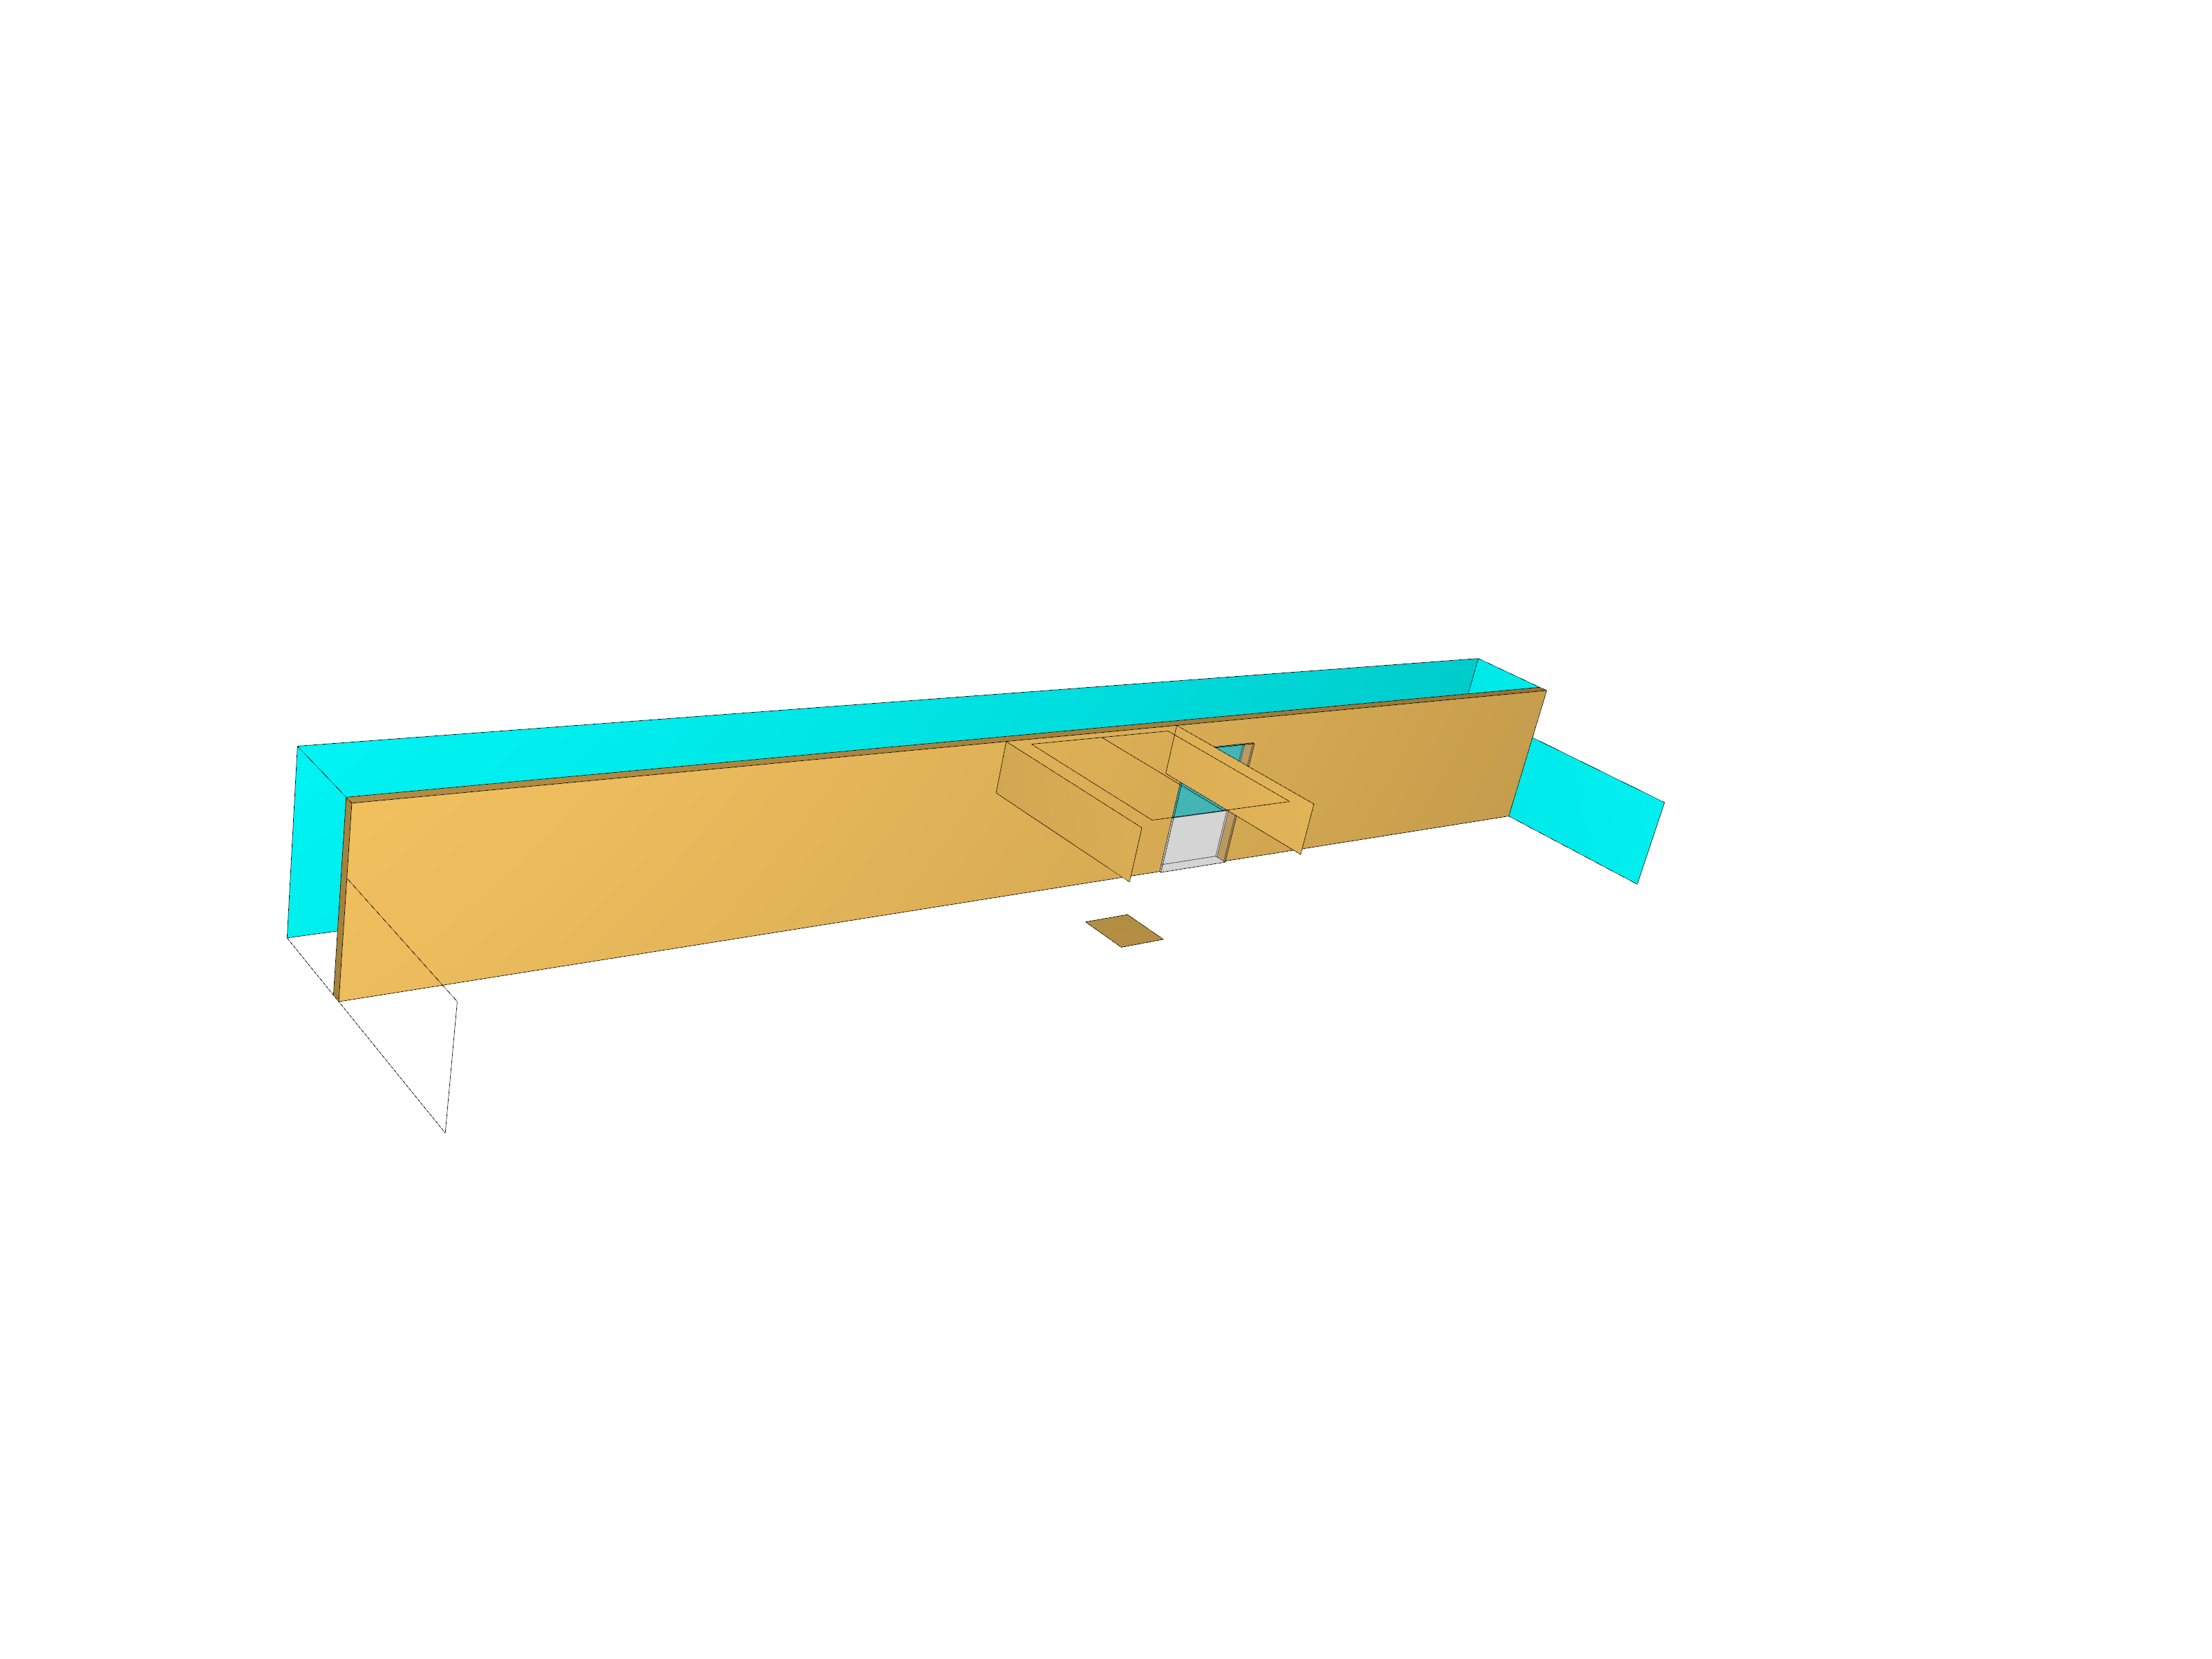
\includegraphics[
    trim=409bp 755bp 786bp 947bp,clip,width=14cm]{../figures/op6_1p12_pyrosim_native.png}};
  \node[anchor=west,font=\sffamily\bfseries\small] at (0,5.52)
    {OP-6\enspace\doorlang{in PyroSim}{原生 PyroSim 视图}};
  \node[anchor=west] at (0,4.95) (outer)
    {\doorlang{Exterior open boundary}{门外计算域的开放边界}};
  \draw[leader] (outer.east) -- ++(.25,0) -- (5.25,4.18);
  \fill[ink] (5.25,4.18) circle (1.25pt);
  \node[anchor=west] at (8,.9) (burner) {\doorlang{Floor burner}{地面火源}};
  \draw[leader] (burner.north) -- (8.46,1.98);
  \fill[ink] (8.46,1.98) circle (1.25pt);
  \node[anchor=west] at (10.8,1.66) (rdoor) {\doorlang{R1 opening}{R1 侧墙开口}};
  \draw[leader] (rdoor.west) -- ++(-.42,0) -- (9.22,2.96);
  \fill[ink] (9.22,2.96) circle (1.25pt);
\end{tikzpicture}
